\documentclass{article}
\usepackage[en]{ukon-infie}
\usepackage[utf8]{inputenc}
\usepackage{algorithm2e}
\usepackage{amsmath}
\usepackage{graphicx}
\usepackage{hyperref}
% kann de oder en sein
% kann bubble break, topexercise sein

\Names{Jonas Probst, Simon Giebenhain}
\Lecture[AnaVis]{Analyse und Visualisierung von Informationen}
\Term{WS 2017/18}

\begin{document}
    \begin{ukon-infie}[17.01.18]{9}

        \begin{exercise}[p=4]{Information Visualization Reference Model}  
       	Step 1: Transform Raw Data to useful Data Tables by standard filtering and data cleaning methods.\\\\
       	Step 2: Decide which data should be used in the later visualization and perform necessary transformations.\\\\
       	Step 3: Decide which visualization methods should be used and implement them using the data from previous steps.\\\\
       	Step 4: Evaluate you visualization and if necesarry adjust previous steps.
    	

		\end{exercise}
		
		
		\begin{exercise}[p=8]{Judging Visualizations}
		\textbf{The Good Visualization}\\\\
		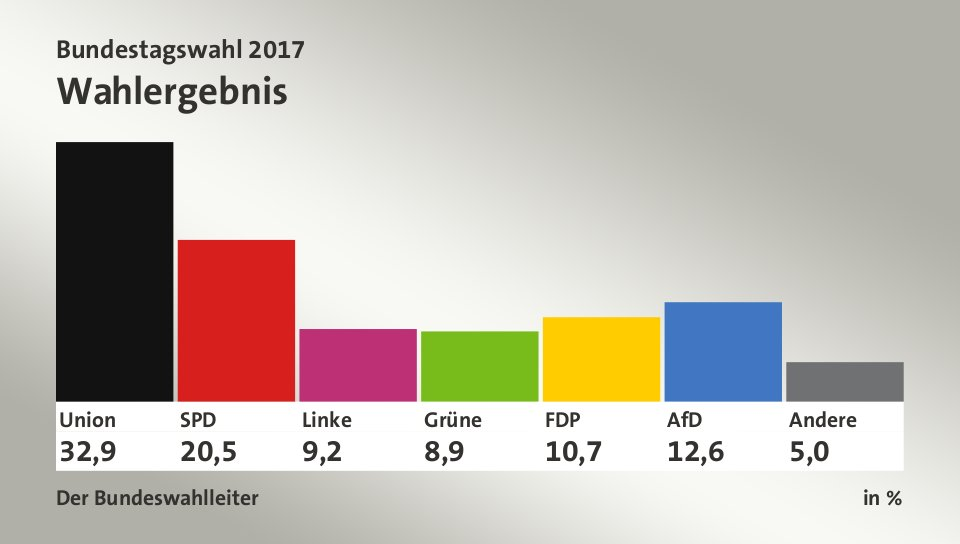
\includegraphics[scale=0.5]{good_example.jpg}\\
		Source: \url{https://wahl.tagesschau.de/wahlen/2017-09-24-BT-DE/index-content.shtml}\\\\
		The visualization shows the results of the last Bundestagswahl in Germany. It's a simple bar chart, with one bar for each party.\\
		\newpage
		Used visual variables are:\\
		\textbf{length:} to directly show the percantages and give a visual way of comparing them.\\
		\textbf{colour:} matching the respective parties.\\
		\textbf{position:} matching the results of the last election.\\\\
		Used Gestalt Laws:\\
		\textbf{Proximity:} Party names and percentages are connected to the bars above them.\\\\
		The visualization is very simple and easy to understand and doesn't contain unnecessary information or try to influence the opininon of the reader in some way. 
		Only the ordering of the parties could be changed after the election finished, from strongest to weakest, as the ordering right now is from the last election.\\\\\\
		
		
		\textbf{The Bad Visualization}\\\\
		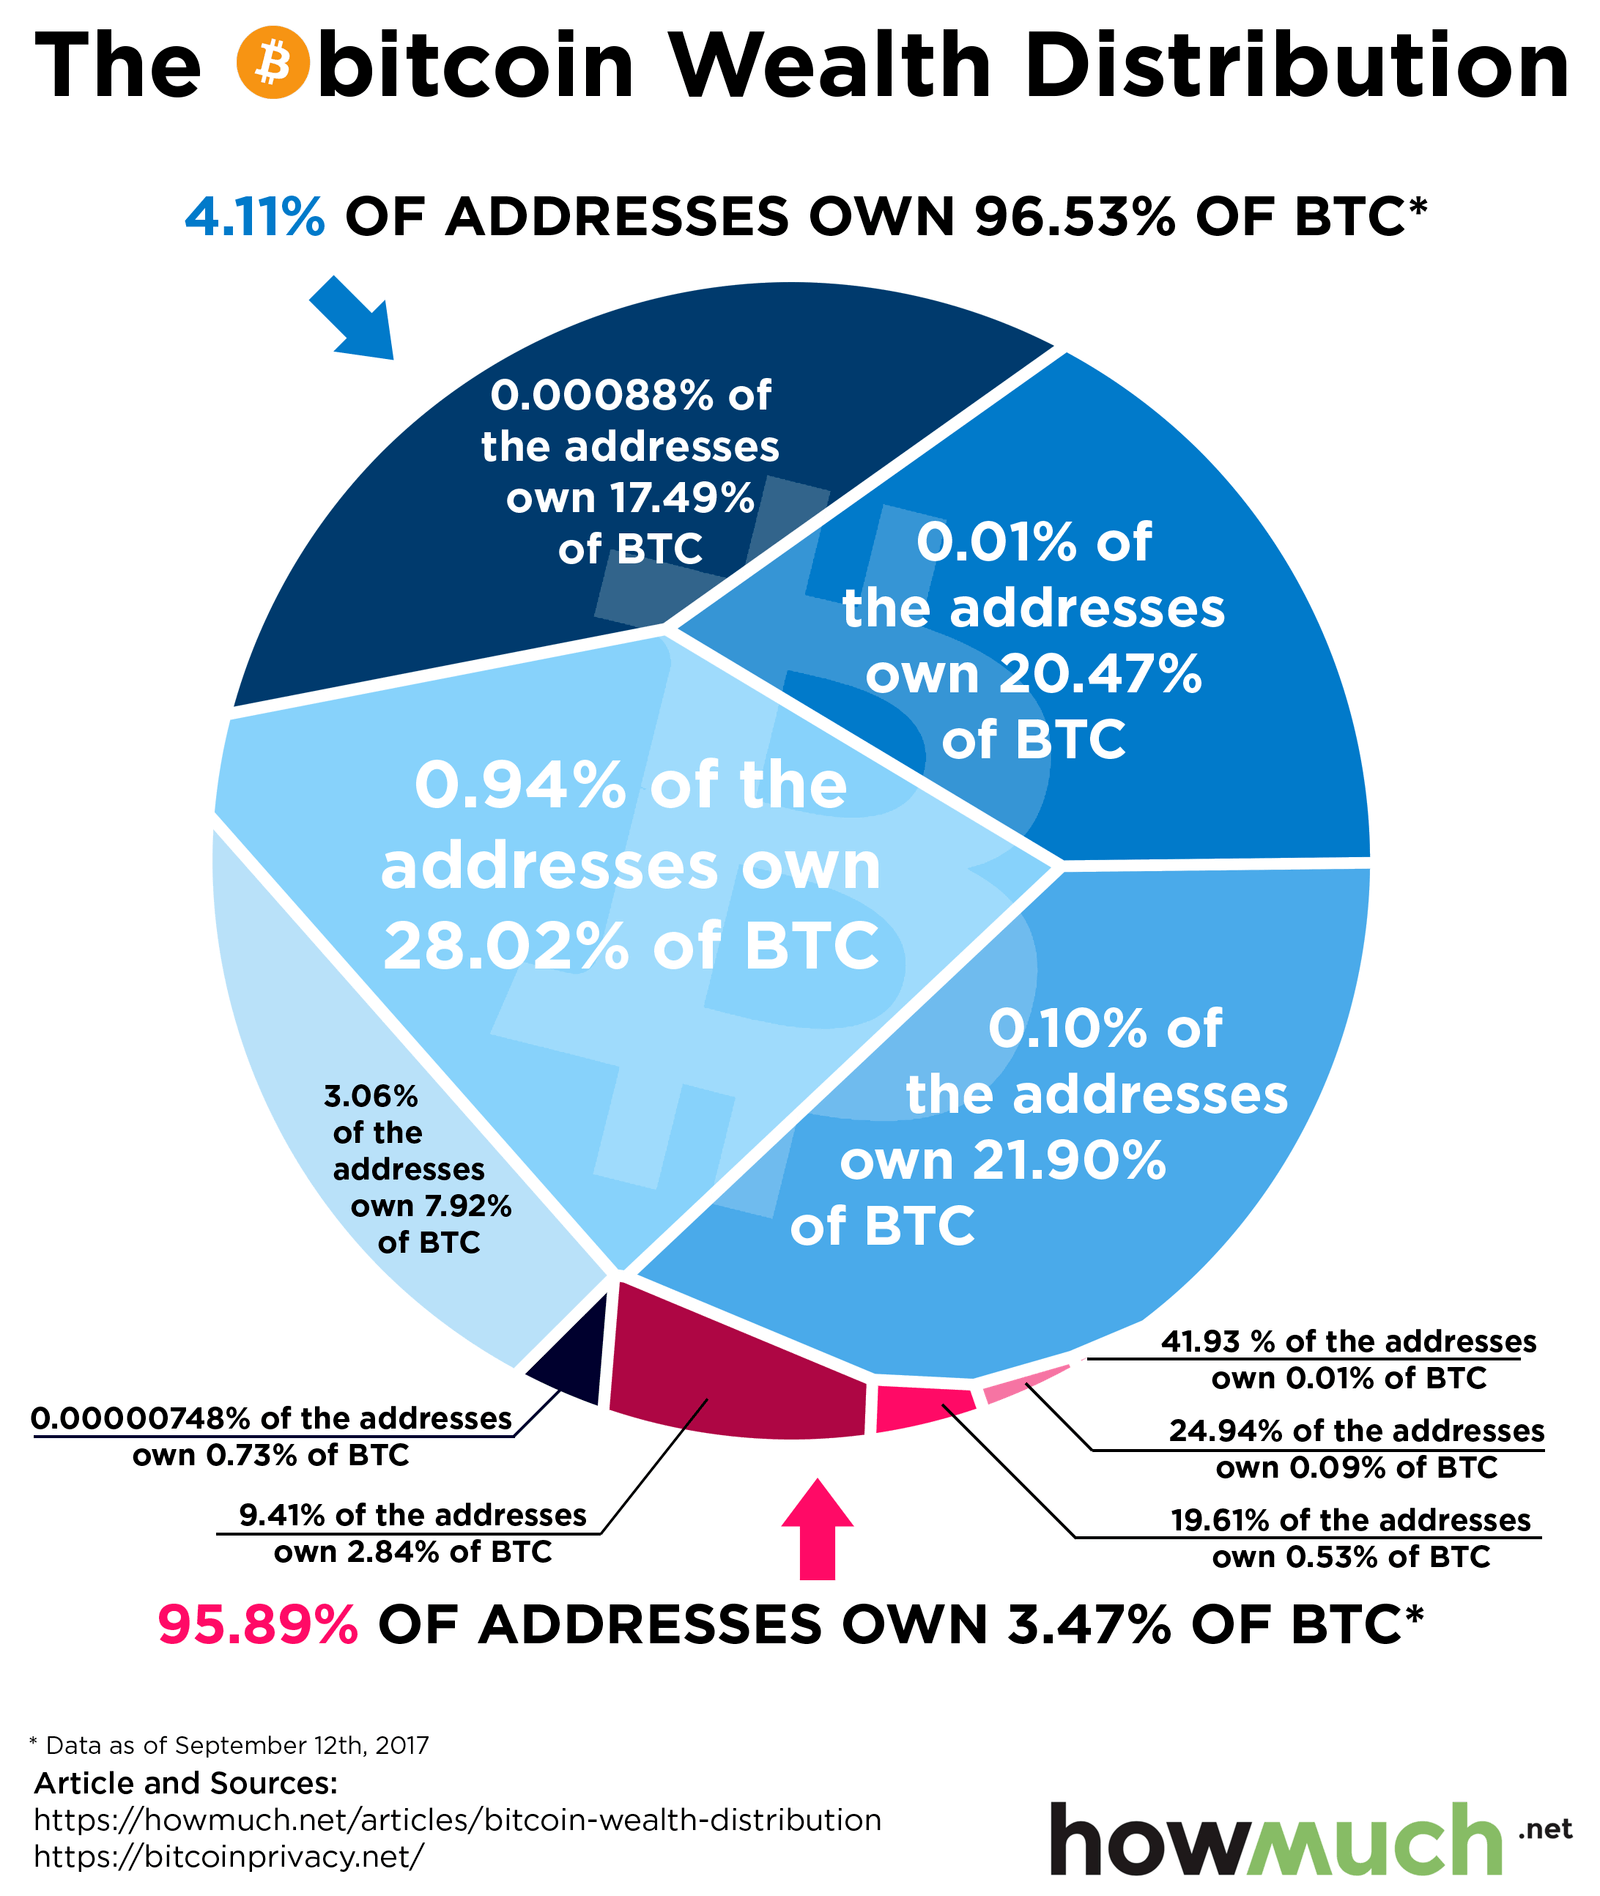
\includegraphics[scale=0.2]{bad_example.png}\\
		Source: \url{https://howmuch.net/articles/bitcoin-wealth-distribution}\\\\
		The visualization shows the wealth distribution of bitcoin in some kind of "pie chart" where the whole pie is the total amount of bitcoins in circulation. The chart is split up in seemingly arbitrary portions which represent how much bitcoin a certain percantage of addresses holds. \\\\
		\newpage
		Used Visual Variables are:\\
		\textbf{area:} to represent amount of bitcoin\\
		\textbf{colour:} to represent the order of the pieces.\\
		\textbf{density} or intensity of the colours change, the lower the intensity, the more addresses are contained in the segment.\\\\
		Used Gestalt Laws are: \\
		\textbf{Proximity}: The text in a segment belongs to the segment.\\
		\textbf{Connectedness}: Percentages for smaller segments are connected with lines.\\
		\textbf{Continuity}: The seperate segments are perceived as a circle.\\\\
		The visualization in general is really unintuitive, because all percentages are seemingly chosen randomly which makes it difficult to compare multiple segments. Without the caption you would not get the information that 4.11\% of the addresses hold 96.53\% of BTC. The colours are not easily interpreted and the change in intensity doesn't make sense at first glance. \\\\
		
 
		Another way of visualizin the BTC distribution would be a Graph. This sketch is really simple, one could for example add a point to the graph at the 96\% mark of the addresses, to highlight the information of the pie chart that 4\% of Addresses own 96.5\% of BTC.\\
		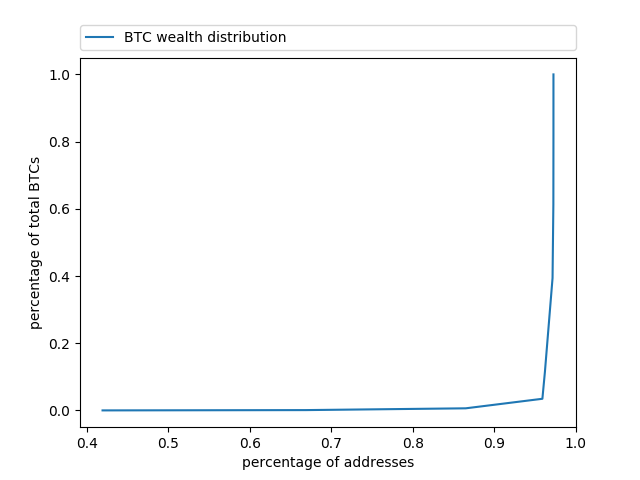
\includegraphics[scale=1]{BTC_wealth_distribution.png}
		\end{exercise}
		\newpage
		\begin{exercise}[p=10]{Data Analysis and Visualization Task}
		\textbf{Preprocessing:}
		
		\begin{itemize}
		\item Remove id
		\item set empty income to 0
		\item normalize income, age
		\item ask what save\_act, current\_act and pep mean, if noone knows, delete them
		\end{itemize}
		
		Perform PCA. If results are good, reduce dimensionality.\\\\
		
		Play around with different kinds of plots, e.g. a scatterplot with Age vs. Income where the colour of the point maches the region. Look for outliers and trends in the data.\\\\	
		
		\textbf{Clustering:}
		\begin{itemize}
		\item Design a distance measure which incorporates nominal and numeric data.
		\item Try different clustering algorithms. Compare results by reducing the visualization to a 3D plot (with PCA).
		\item For best method, adjust and refine clustering.
		\end{itemize}
		
		\textbf{Assoiciation Rules:}
		\begin{itemize}
		\item Group age and income in groups so association rules can be found.
		\item Find rules using FP-Growth. Adjust confidence and support based on first results. Also try different groupings for age and income.
		
		\end{itemize}
		
		
		
		\textbf{Visualization:}\\
		Summarize knowlede gained in previous steps in different kinds of plots.  One could be a scatterplot with age on one axis and income on the other (only numeric values), where the colour, shape and size of the points show information as well. Another one would probably be a 3D Visualization for the Clustering with PCA.
				
		\end{exercise}
		
		
\end{ukon-infie}
\end{document}
